\begin{frame}{Scaling Laws for LLMs}
  \begin{itemize}
    \item[\textcolor{red}{$\blacktriangleright$}] \textbf{Kaplan et al. (2020):} ``Scaling Laws for Neural Language Models''
    \item[\textcolor{red}{$\blacktriangleright$}] Performance improves predictably with:
      \begin{itemize}
        \item More parameters
        \item More compute
        \item Larger datasets
      \end{itemize}
    \item[\textcolor{red}{$\blacktriangleright$}] \textbf{Optimal allocation of compute:} Train bigger models with less data, rather than small models with lots of data.
    \item[\textcolor{red}{$\blacktriangleright$}] \textbf{Implication:} LLMs like GPT-3 (175B), GPT-4 (est.\ $>$500B) are products of scaling laws.
  \end{itemize}
\end{frame}

\begin{frame}{Scaling in GPT-2}
  \begin{itemize}
    \item Scaling improves the perplexity of the LM and improves performance
  \end{itemize}
  \begin{center}
    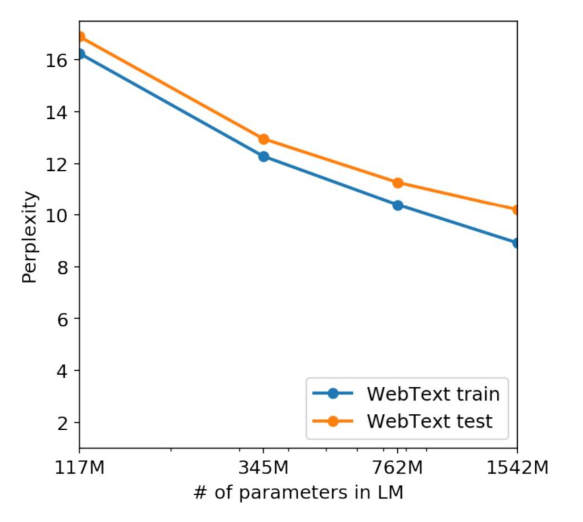
\includegraphics[width=0.45\linewidth, height=0.45\paperheight, keepaspectratio]{images/large-language-models/llm_scaling_perplexity_vs_parameters.png}

    {\scriptsize Source: Radford et al., ``Language Models are Unsupervised Multitask Learners'' (GPT-2), OpenAI 2019, Fig.~4.}
  \end{center}
\end{frame}

\begin{frame}{Why is this interesting? Look at data scaling}
  \begin{itemize}
    \item We know that typical scaling effects look like this when we increase the amount of training data
  \end{itemize}
  \begin{center}
    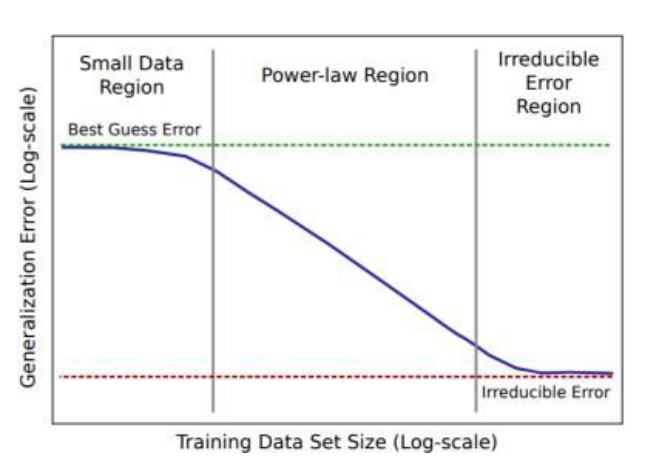
\includegraphics[width=0.45\linewidth, height=0.45\paperheight, keepaspectratio]{images/large-language-models/llm_generalization_error_regions.png}

    {\scriptsize Source: Hestness et al., ``Deep Learning Scaling is Predictable, Empirically'', 2017, Fig.~6.}
  \end{center}
\end{frame}

\begin{frame}{Why is this interesting? Look at data scaling}
  \begin{itemize}
    \item Loss and dataset size is linear on a log-log plot
    \item This is ``power-law scaling''
  \end{itemize}
  \begin{center}
    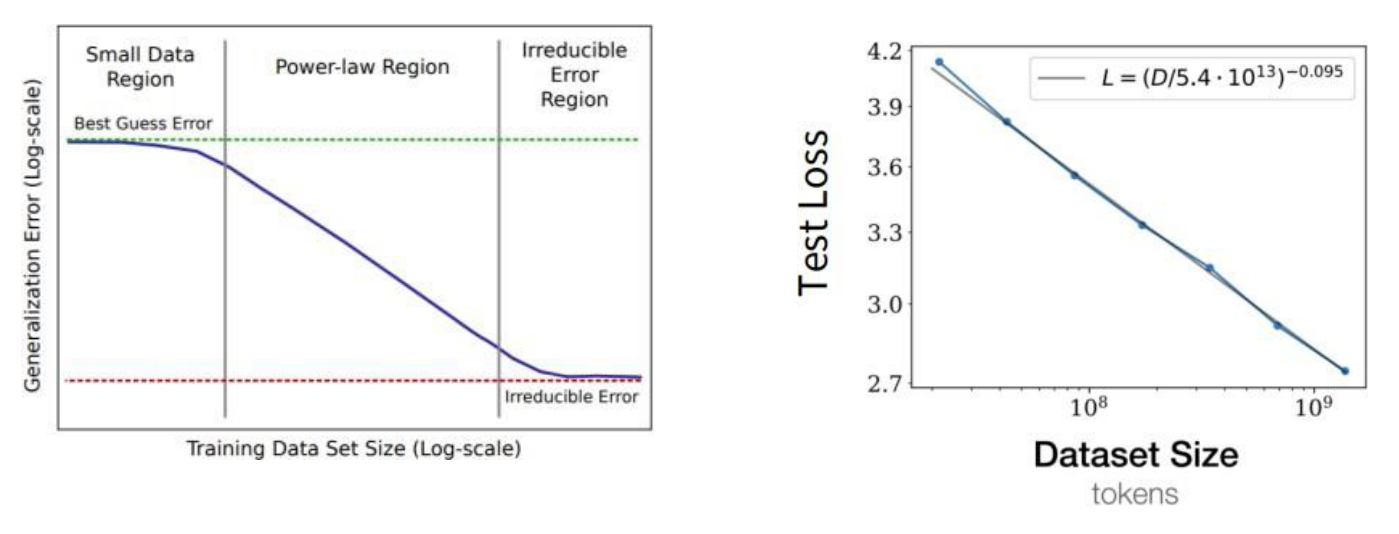
\includegraphics[width=0.7\linewidth, height=0.7\paperheight, keepaspectratio]{images/large-language-models/llm_scaling_test_loss_vs_dataset_size.png}

    {\scriptsize Source: Hestness et al., 2017, Fig.~6 (left); Kaplan et al., ``Scaling Laws for Neural Language Models'', 2020, Fig.~1 (right).}
  \end{center}
\end{frame}

\begin{frame}{Scaling -- \textnormal{(Kaplan, 2020)}}
  \begin{itemize}
    \item Can we understand scaling by positing scaling laws?
    \item With scaling laws, we can make decisions on architecture, data,\\ and hyperparameters by training smaller models.
    \item \textbf{OpenAI Study:} \href{https://arxiv.org/abs/2001.08361}{\textcolor{red}{Scaling Laws for Neural Language Models}} (\href{https://arxiv.org/abs/2001.08361}{Kaplan et al., 2020})
  \end{itemize}
\end{frame}

\begin{frame}{Scaling -- \textnormal{(Kaplan, 2020)}}
  \begin{itemize}
    \item \textbf{OpenAI Study:} \href{https://arxiv.org/abs/2001.08361}{\textcolor{red}{Scaling Laws for Neural Language Models}} (\href{https://arxiv.org/abs/2001.08361}{Kaplan et al., 2020})
  \end{itemize}
  \vspace{0.6em}
  \textbf{Key Findings:}
  \begin{itemize}
    \item Performance depends strongly on scale, and only weakly on the model shape.
    \item Larger models are more sample-efficient.
    \item Smooth power laws $(y = ax^b)$ observed between empirical performance and:
      \begin{itemize}
        \item $N$ -- number of parameters
        \item $D$ -- dataset size
        \item $C$ -- compute
      \end{itemize}
  \end{itemize}
\end{frame}

\begin{frame}{Compute-Optimal Scaling -- \textnormal{(Hoffmann, 2022)}}
  \begin{itemize}\itemsep0.25em
    \item Kaplan's split favours parameters: $10\times$ the compute buys $5.5\times$ the parameters but only $1.8\times$ the tokens.
    \item \textbf{DeepMind Study:} \href{https://arxiv.org/abs/2203.15556}{\textcolor{red}{Training Compute-Optimal Large Language Models}} (\href{https://arxiv.org/abs/2203.15556}{Hoffmann et al., 2022}) refit the laws over 400+ models (70M--16B parameters, 5B--500B tokens).
    \item \textbf{Result:} $N$ and $D$ should scale \emph{equally}: double the model, double the tokens, or about 20 training tokens per parameter.
    \item \textbf{Chinchilla vs.\ Gopher,} at the same compute budget:
      \begin{itemize}
        \item Gopher: 280B parameters, 300B tokens
        \item Chinchilla: 70B parameters, 1.4T tokens, and it outperforms Gopher
      \end{itemize}
    \item \textbf{Takeaway:} those models were undertrained, not too small. A scaling law is an empirical fit, and can be refit when the experiment is run more carefully.
  \end{itemize}
\end{frame}

\begin{frame}{Scaling Effects}
  \begin{itemize}
    \item The effect of some hyperparameters on large language models (LMs) can be predicted before full training: optimizer choice (Adam vs.\ SGD), model depth, and architecture (LSTM vs.\ Transformer).
  \end{itemize}
  \vspace{0.9em}
  Idea:
  \begin{itemize}
    \item[] \begin{itemize}
      \item Train a few smaller models
      \item Establish a scaling law (e.g., Adam vs.\ SGD scaling law)
      \item Select optimal hyperparameters based on the scaling law prediction
    \end{itemize}
  \end{itemize}
\end{frame}

\begin{frame}{Model Scaling: GPT-3}
  \centering
  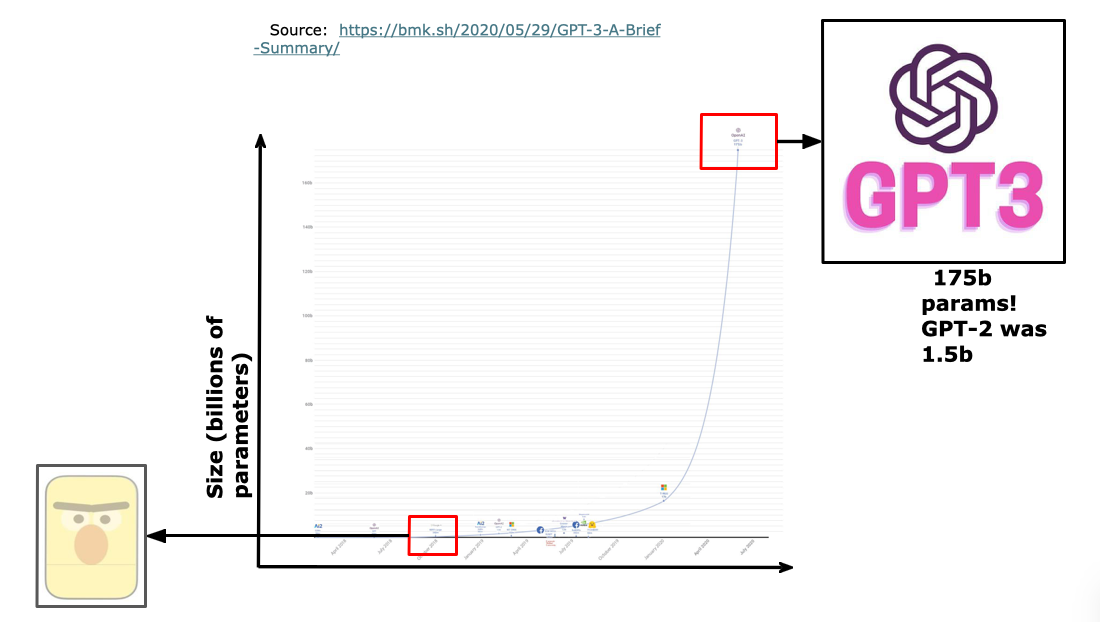
\includegraphics[width=0.60\paperwidth,height=0.60\paperheight,keepaspectratio]{images/large-language-models/llm_model_size_growth_gpt3.png}

  {\scriptsize Source: Leo Gao, ``Why GPT-3 Matters'', 2020 (chart edited by WillStats).}
\end{frame}

\begin{frame}{Emergent Abilities with GPT-3 -- \textnormal{Wei et al., 2022}}
  \begin{itemize}
    \item \textbf{Emergent abilities:}
      \begin{itemize}
        \item Not present in smaller models but is present in larger models
        \item Do LLMs like GPT-3 have these?
      \end{itemize}
    \vspace{1em}
    \item \textbf{Findings:}
      \begin{itemize}
        \item GPT-3 trained on text can do arithmetic problems like addition and subtraction
        \item Different abilities ``emerge'' at different scales
      \end{itemize}
  \end{itemize}
\end{frame}

\begin{frame}{Emergent Abilities with GPT-3 -- \textnormal{Wei et al., 2022}}
  \begin{itemize}
    \item \textbf{Emergent abilities:}
      \begin{itemize}
        \item Not present in smaller models but is present in larger models
        \item Do LLMs like GPT-3 have these?
      \end{itemize}
    \vspace{1em}
    \item \textbf{Findings:}
      \begin{itemize}
        \item GPT-3 trained on text can do arithmetic problems like addition and subtraction
        \item Different abilities ``emerge'' at different scales
        \item \textcolor{red}{Model scale is \textbf{not} the only contributor to emergence} -- for 14 BIG-Bench tasks, LaMDA 137B and GPT-3 175B models perform at near-random, but PaLM 62B achieves above-random performance
        \item Problems LLMs can’t solve today may be emergent for future LLMs
      \end{itemize}
  \end{itemize}
\end{frame}
